% =========================
% DOCUMENT CLASS
% =========================
\documentclass[a4paper,12pt,openany]{report}

% =========================
% PACKAGES
% =========================
\usepackage{graphicx}
\usepackage{multirow}
\usepackage{amsmath,amssymb,amsfonts}
\usepackage{amsthm}
\usepackage{mathrsfs}
\usepackage{xcolor}
\usepackage{textcomp}
\usepackage{booktabs}
\usepackage{algorithm}
\usepackage{algpseudocode}
\usepackage{listings}
\usepackage[a4paper, top=2cm, bottom=2cm, left=2.5cm, right=2.5cm]{geometry}

% Show deeper section levels
\setcounter{secnumdepth}{3}
\setcounter{tocdepth}{3}

% Section indentation matching reference template
\usepackage{titlesec}
\titleformat{\section}[hang]{\bfseries}{\thesection}{1em}{}
\titlespacing{\section}{0pt}{\parskip}{0.5\parskip}

\titleformat{\subsection}[hang]{\bfseries}{\thesubsection}{1em}{}
\titlespacing{\subsection}{30pt}{\parskip}{0.5\parskip}

\titleformat{\subsubsection}[hang]{\bfseries}{\thesubsubsection}{1em}{}
\titlespacing{\subsubsection}{50pt}{\parskip}{0.5\parskip}

% =========================
% BEGIN DOCUMENT
% =========================
\begin{document}

% =========================
% CUSTOM TITLE PAGE
% =========================
\begin{titlepage}

\begin{center}

{\large \textbf{HANOI UNIVERSITY OF SCIENCE AND TECHNOLOGY}}\\[2cm]

{\Huge \textbf{GRADUATION THESIS}}\\[1.5cm]

{\Large Edge-based Traffic Prediction via Federated Learning}\\[2cm]

{\large \textbf{LUU QUOC KHANH}}\\
{\large enter email here}\\[0.3cm]

{\large \textbf{DOAN NGUYEN NGOC SON}}\\
{\large enter email here}\\[0.5cm]

{\large Program: Global ICT}\\[2cm]

\begin{flushleft}
\textbf{Supervisor:} Associate Professor PHAM VAN HAI
\end{flushleft}

\vspace{1cm}

\begin{flushleft}
\textbf{Department:} Computer Engineering
\end{flushleft}

\begin{flushleft}
\textbf{School:} School of Information and Communications Technology
\end{flushleft}

\vfill

{\large HANOI, 12/2025}

\end{center}

\end{titlepage}

% =========================
% TABLE OF CONTENTS
% =========================
\tableofcontents

% =========================
% CHAPTER 1
% =========================
\chapter{INTRODUCTION}

\section{Problem Statement}

\section{Background and Problems}
\subsection{Privacy Risks of Centralized Traffic Systems}

\section{Privacy vs. Accuracy: The Case for Federated Learning}
\subsection{Quantifying the Accuracy Loss}
\subsection{Concrete Privacy Benefits}
\subsection{When Federated Learning Is the Right Choice}

\section{Objectives}

\section{Contributions}

\section{Organization}

% =========================
% CHAPTER 2
% =========================
\chapter{REQUIREMENT SURVEY AND ANALYSIS}

\section{Traffic Flow Prediction}
\subsection{Traditional Approaches}
\subsection{Deep Learning Approaches}

\section{Federated Learning in Intelligent Transportation Systems}

\section{State-of-the-Art in Federated Traffic Prediction}
\subsection{Spatial-Temporal Modeling in FL}
\subsection{Heterogeneity and Personalization}
\subsection{Privacy and Security Enhancements}

\section{Theoretical Background}
\subsection{Long Short-Term Memory (LSTM)}
\subsection{Federated Averaging (FedAvg)}

% =========================
% CHAPTER 3
% =========================
\chapter{METHODOLOGY}

\section{Overview}

\section{Federated Learning Framework}

\section{Collaborative Training Process}

\section{System Architecture and Components}
\subsection{Traffic Data Environment}
\subsection{Data Streaming Layer}
\subsection{Edge Clients}
\subsection{Federated Learning Server}
\subsection{Problem Definition}
\subsection{Multi-Horizon LSTM Architecture}

\section{Network Topology Analysis for Edge Placement}
\subsection{Louvain Clustering for Community Detection}
\subsection{Centrality-Based Representative Selection}
\subsection{Benefits of Topology-Based Placement}

\section{Federated Aggregation Algorithm}

\section{Communication Protocol and Efficiency}
\subsection{Asynchronous Communication}
\subsection{Bandwidth Efficiency Gains}

% =========================
% CHAPTER 4
% =========================
\chapter{EXPERIMENT EVALUATION}

% =========================
% SECTION 4.1
% =========================
\section{Experimental Setup}

\subsection{Simulation Environment}

The experiment is performed using the following software stack:
\begin{itemize}
    \item \textbf{Traffic simulation:} SUMO (Simulation of Urban Mobility) v1.18.0
    \item \textbf{Federated Learning:} Flower Framework v1.5.0
    \item \textbf{Deep Learning Library:} PyTorch v2.0.1
    \item \textbf{Dashboard:} Streamlit-based dashboard
\end{itemize}

The core logic of the three main system loops is described by the pseudo-code below.

\begin{algorithm}[H]
\caption{SUMO Simulation Loop}
\begin{algorithmic}[1]
\State Initialize SUMO simulation with network, route, and config files
\State Open WebSocket server
\While{simulation\_step $<$ MAX\_STEPS}
    \State Execute one simulation step
    \State Extract traffic features (speed, count, density) per region
    \For{each subscribed edge client}
        \State Send traffic data via WebSocket
    \EndFor
    \State Advance to next timestep
\EndWhile
\State Shut down simulation and close WebSocket server
\end{algorithmic}
\end{algorithm}

\begin{algorithm}[H]
\caption{Edge Client Loop}
\begin{algorithmic}[1]
\State Initialize edge client with assigned region IDs
\State Connect to SUMO server and subscribe to assigned regions
\While{running}
    \If{data received from SUMO}
        \State Parse message and append to local buffer
    \EndIf
    \If{enough data to train}
        \State Sample training data from buffer
        \For{each epoch}
            \State Train local model on sampled data
        \EndFor
        \State Update local model weights
    \EndIf
    \If{FL round triggered}
        \State Receive global parameters from FL server
        \State Update local model with global parameters
        \State Train local model for FL round
        \State Send local update to FL server
        \State Evaluate on local data and send metrics to FL server
    \EndIf
\EndWhile
\end{algorithmic}
\end{algorithm}

\begin{algorithm}[H]
\caption{Federated Learning Server Loop}
\begin{algorithmic}[1]
\State Initialize global model and bind to server address
\For{each round $r = 1$ \textbf{to} MAX\_ROUNDS}
    \State Select a fraction of available edge clients
    \For{each selected client}
        \State Send current global model parameters
    \EndFor
    \For{each selected client}
        \State Receive local model update
    \EndFor
    \State Aggregate all updates using FedAvg:
    \[
        w_{\text{global}} \leftarrow \sum_{k=1}^{K} \frac{n_k}{n}\, w_k
    \]
    \State Update global model with aggregated parameters
    \State Collect and aggregate validation metrics from clients
    \State Log round metrics to disk
\EndFor
\end{algorithmic}
\end{algorithm}

\subsection{Benchmark Dataset Description}

This report uses data collected from two widely adopted benchmark traffic datasets:
PeMS-BAY and METR-LA.

\begin{figure}[H]   %figure 4.1
    \centering
    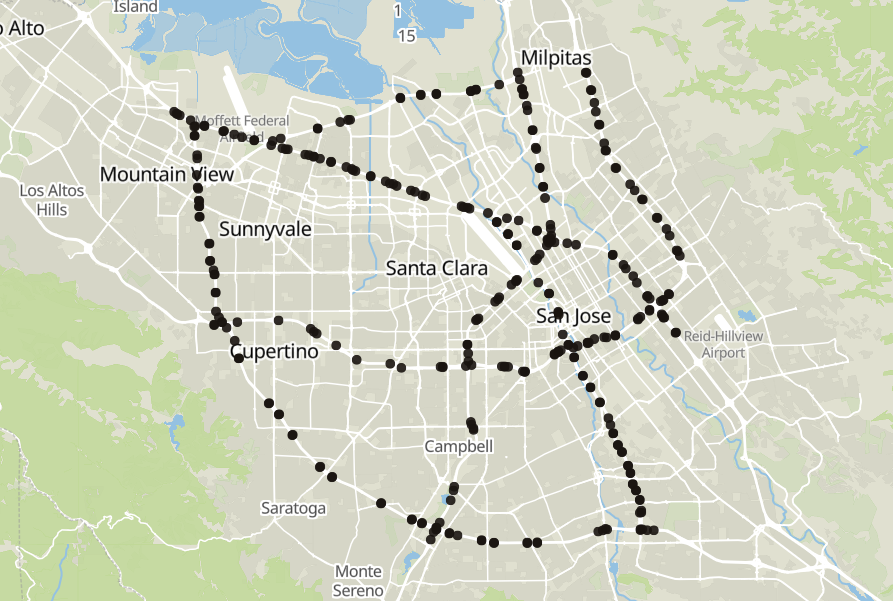
\includegraphics[width=1.0\textwidth]{Figure/pems-bay-spatial.png}
    \caption{PEMS-BAY Dataset Spatial}
    \label{fig:pems-bay-dataset}
\end{figure}

The \textbf{PeMS-BAY} dataset contains traffic data from 325 sensors in the Bay Area,
collected over six months (January--May 2017) at 5-minute intervals. Missing values
are handled using linear interpolation, and the data is normalized using Z-score
normalization to improve model performance.

\begin{figure}[H]
    \centering
    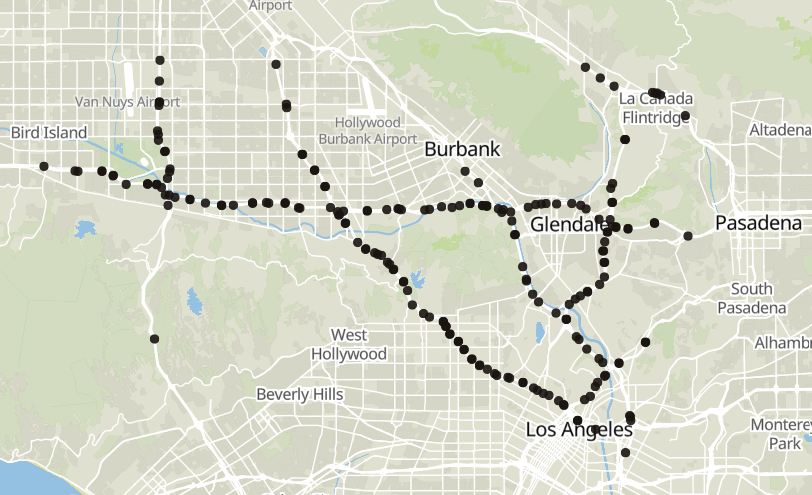
\includegraphics[width=1.0\textwidth]{Figure/metr-la-spatial.png}
    \caption{METR-LA Dataset Spatial}
    \label{fig:metr-la-dataset}
\end{figure}

The \textbf{METR-LA} dataset consists of traffic data from 207 sensors across Los Angeles,
collected over four months at 5-minute intervals. It reflects highly congested urban and
freeway conditions. Missing values (9.93\%) are filled using spatio-temporal
interpolation, and the data is normalized using Z-score normalization.


\subsection{Hyperparameters}

Hyperparameters are configuration values set before training that control how a
machine learning model learns from data. The hyperparameters used in this experiment
are summarized in Table 4.1.

\begin{table}[H]
\centering
\begin{tabular}{|l|l|}
\hline
\textbf{Parameter} & \textbf{Value} \\ \hline
Input Sequence Length ($T_{in}$) & 24 (2 hours) \\ \hline
Prediction Horizons & 3, 6, 12 steps \\ \hline
Batch Size & 32 \\ \hline
Learning Rate & 0.001 \\ \hline
Optimizer & Adam \\ \hline
Local Epochs ($E$) & 5 \\ \hline
FL Rounds ($R$) & 50 \\ \hline
Number of Clients ($K$) & 10 \\ \hline
\end{tabular}
\caption{Experimental Hyperparameters}
\label{tab:hyperparams}
\end{table}

\subsection{SUMO Simulation Demo}

\subsubsection*{a. SUMO Network Configuration}

The SUMO simulation is set up using real-world road network data from OpenStreetMap.
The network includes various road types such as highways, arterial roads, and local
streets, covering a large urban area with many intersections to reflect realistic traffic
conditions. This diversity helps evaluate the model across different traffic scenarios.

The simulation uses SUMO version 1.24.0 and includes specific configurations such as
ignoring route errors for stability, applying adaptive traffic light control based on
congestion, and dynamically rerouting vehicles every 10 seconds. The system also
outputs trip and network statistics for further analysis.

\subsubsection*{b. Multi-Modal Traffic Generation}

\begin{table}[H]
\centering
\begin{tabular}{|l|l|l|}
\hline
\textbf{Vehicle Type} & \textbf{Characteristics} & \textbf{Purpose} \\ \hline
Passenger & High frequency, varying sizes & Commuter traffic, peak patterns \\ \hline
Bus & Lower frequency, large vehicles & Public transit patterns \\ \hline
Truck & Heavy vehicles, restricted routes & Cargo/logistics traffic \\ \hline
Motorcycle  & Agile, small size & Urban mobility dynamics \\ \hline
Bicycle & Slow speed, bike lanes & Active transportation \\ \hline
\end{tabular}
\caption{SUMO Multi-Modal Vehicle Configuration}
\label{tab:sumo_vehicles}
\end{table}

This section describes the use of multi-modal traffic in the simulation, including
different vehicle types such as passenger cars, buses, trucks, motorcycles, and bicycles,
each with distinct characteristics and purposes. This diversity helps create more
realistic traffic conditions.

By incorporating various vehicle types, the system can better simulate real-world
traffic patterns, evaluate model robustness under different conditions, account for
non-recurring events like accidents, and allow edge clients to learn region-specific
traffic behaviors.

\subsubsection*{c. Dataset Streaming via TraCI}

Data is streamed from the SUMO simulation using the TraCI interface. SUMO runs as a
server that allows real-time interaction through TCP, executing simulation steps at
regular intervals (typically every second). During each step, the system extracts data
such as traffic metrics at the edge level (e.g., vehicle count, speed), junction level
(e.g., traffic light status, waiting vehicles), and individual vehicle level (e.g.,
position, speed, trip progress).

\begin{verbatim}
1. Connect to SUMO server via TraCI interface
2. Subscribe to edges and junctions of interest
3. For each simulation step:
   a) Advance SUMO by one timestep
   b) Query subscribed objects for metrics
   c) Aggregate metrics by region/client
   d) Publish via WebSocket to all connected edge clients
   e) Store metrics for offline analysis
\end{verbatim}

\subsubsection*{d. WebSocket Data Publisher}

Traffic data is distributed to edge clients using a WebSocket-based publisher. The
system sends real-time JSON messages at each simulation step (1 Hz), allowing clients
to subscribe to specific road segments relevant to their region. The transmitted data
includes traffic metrics such as vehicle count, speed, density, vehicle types, and road
characteristics.

Example WebSocket message:
\begin{verbatim}
{
  "edge_id": "osm_highway_123",
  "timestamp": "2025-01-17T10:30:45Z",
  "simulation_time": 3645.0,
  "vehicle_count": 24,
  "avg_speed": 12.5,
  "density": 4.8,
  "flow_rate": 345.6,
  "occupancy": 22.3,
  "vehicle_counts_by_type": {
    "passenger": 18,
    "bus": 2,
    "truck": 4
  }
}
\end{verbatim}

\subsubsection*{e. Monitoring Dashboard}

\begin{figure}[H]
    \centering
    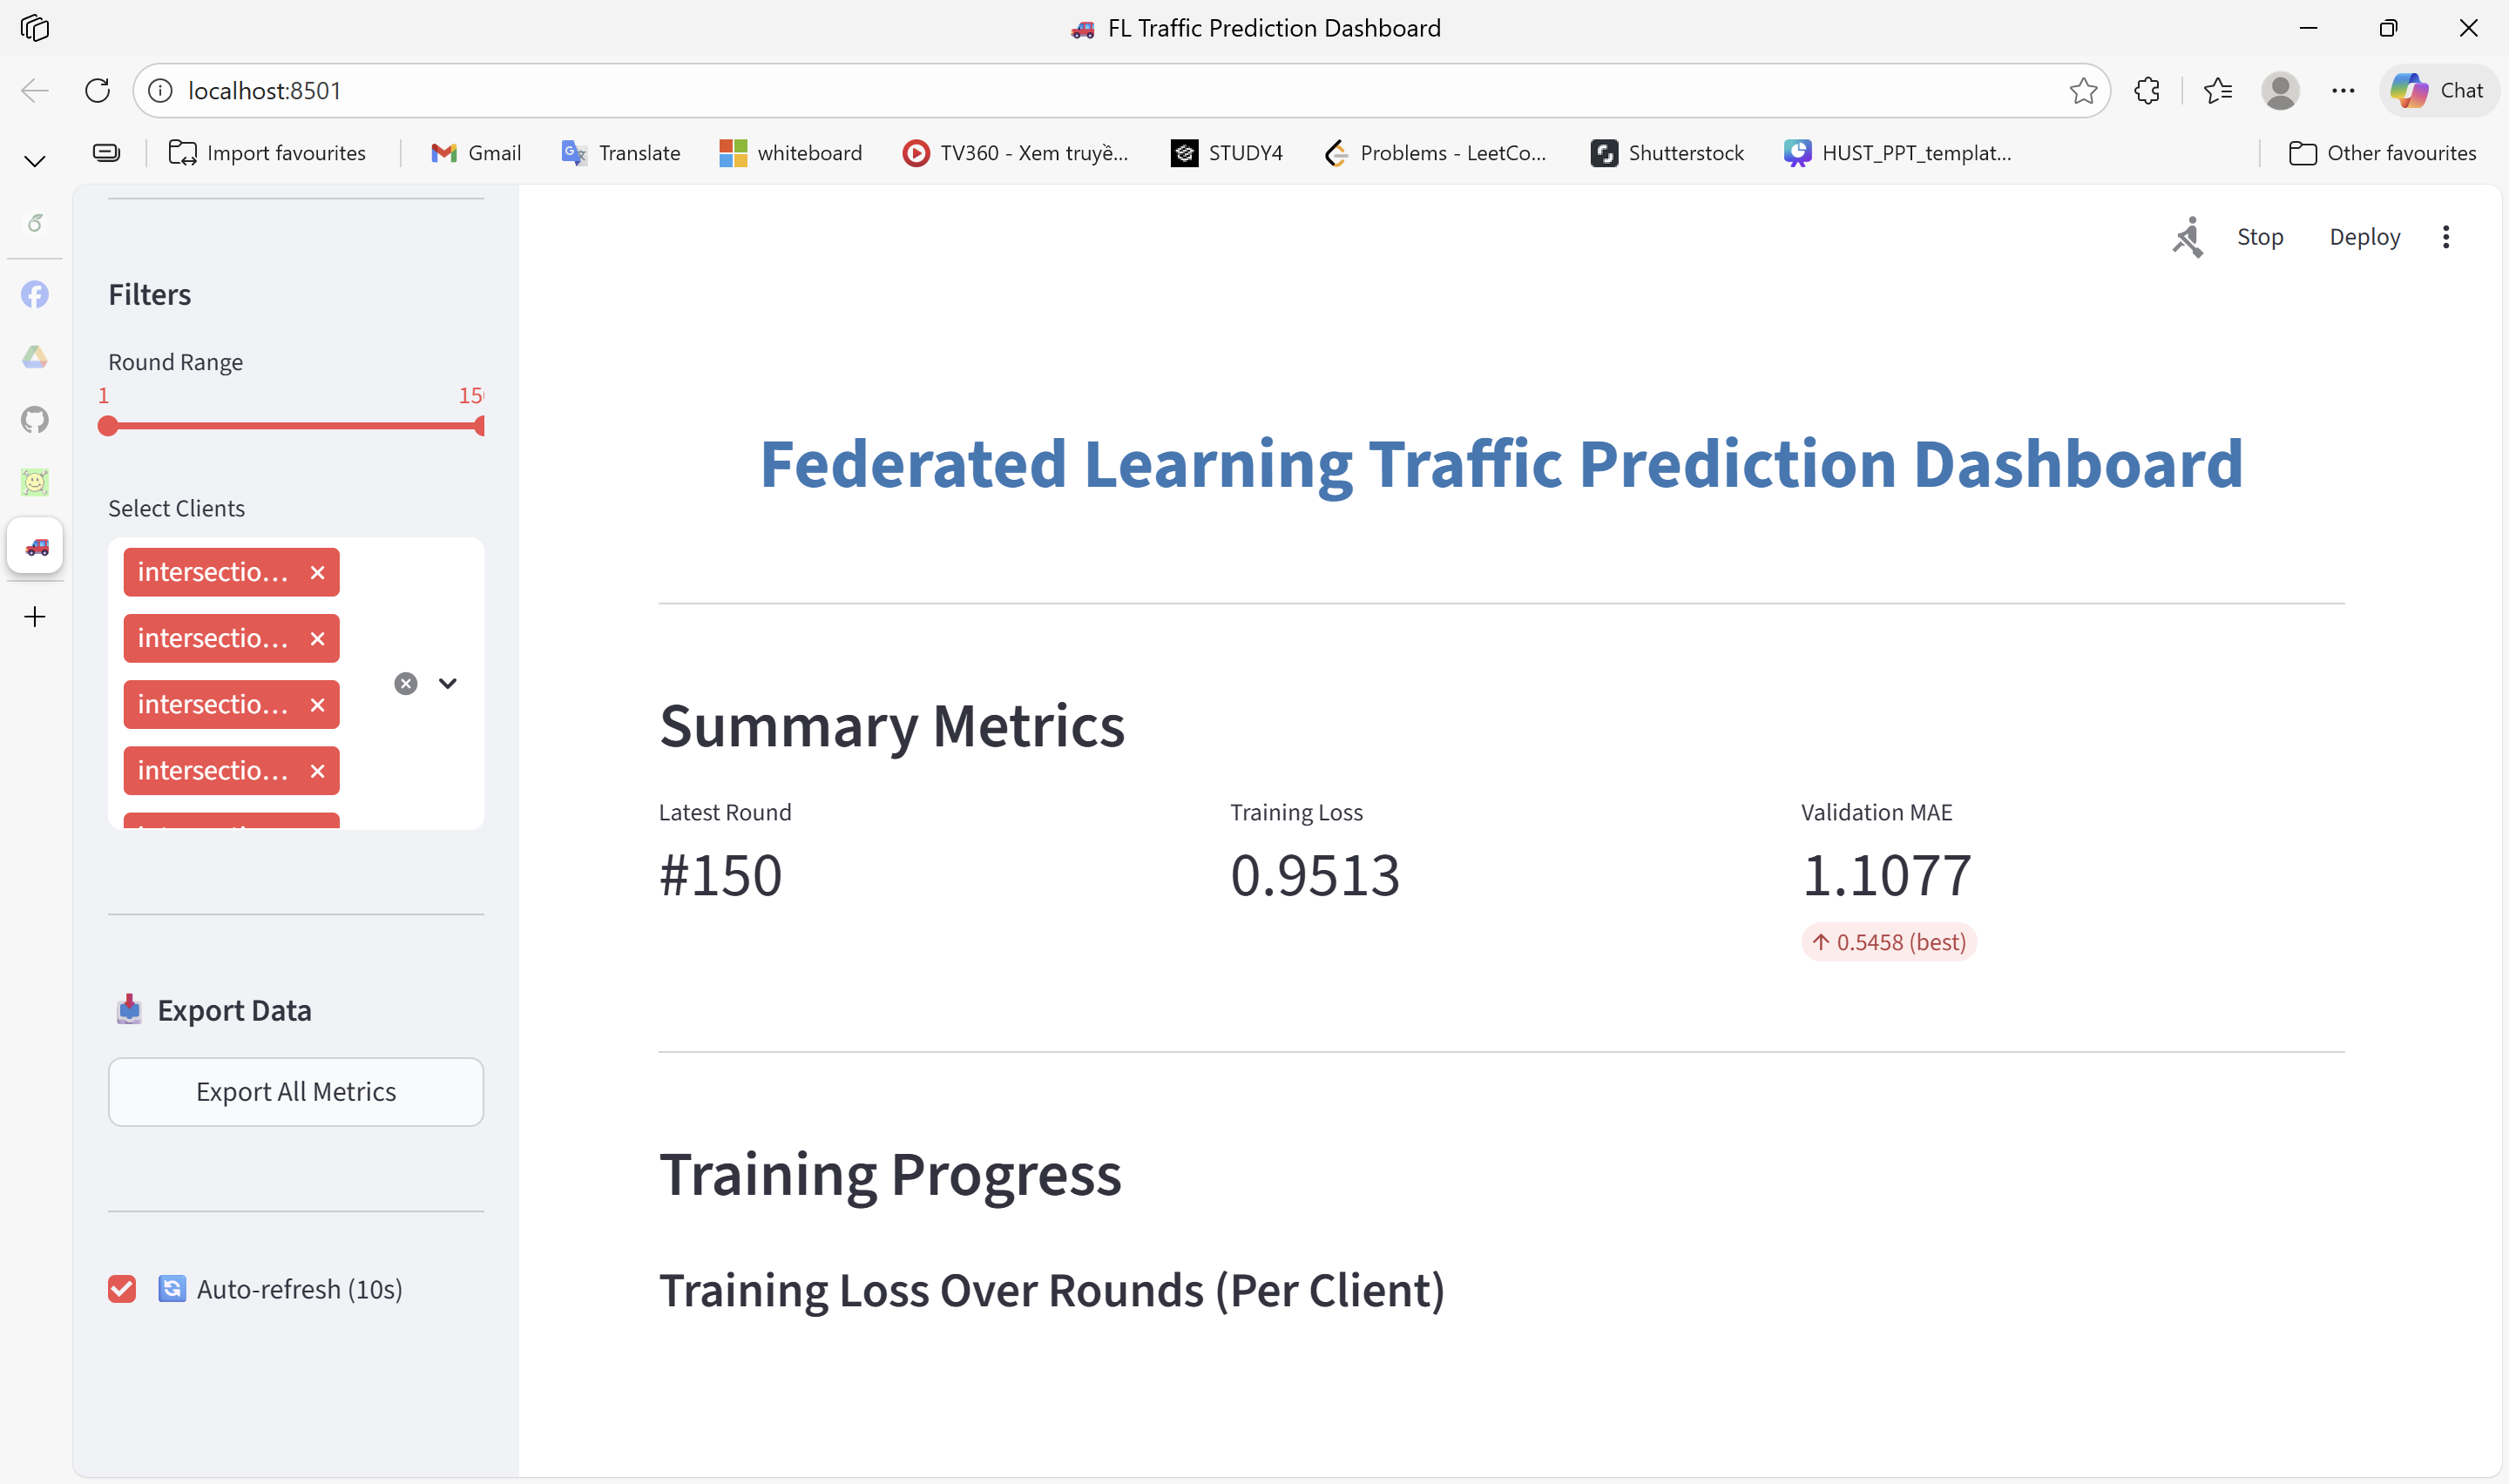
\includegraphics[width=1.0\textwidth]{Figure/dashboard-overview.png}
    \caption{FL Traffic Prediction Dashboard - Summary Metrics. }
    \label{fig:dashboard_overview}
\end{figure}

The data is displayed through a Streamlit-based monitoring dashboard that visualizes
the federated learning process and system performance in real time. It displays key
metrics such as training loss, validation error, and current training round.

\begin{figure}[H]
    \centering
    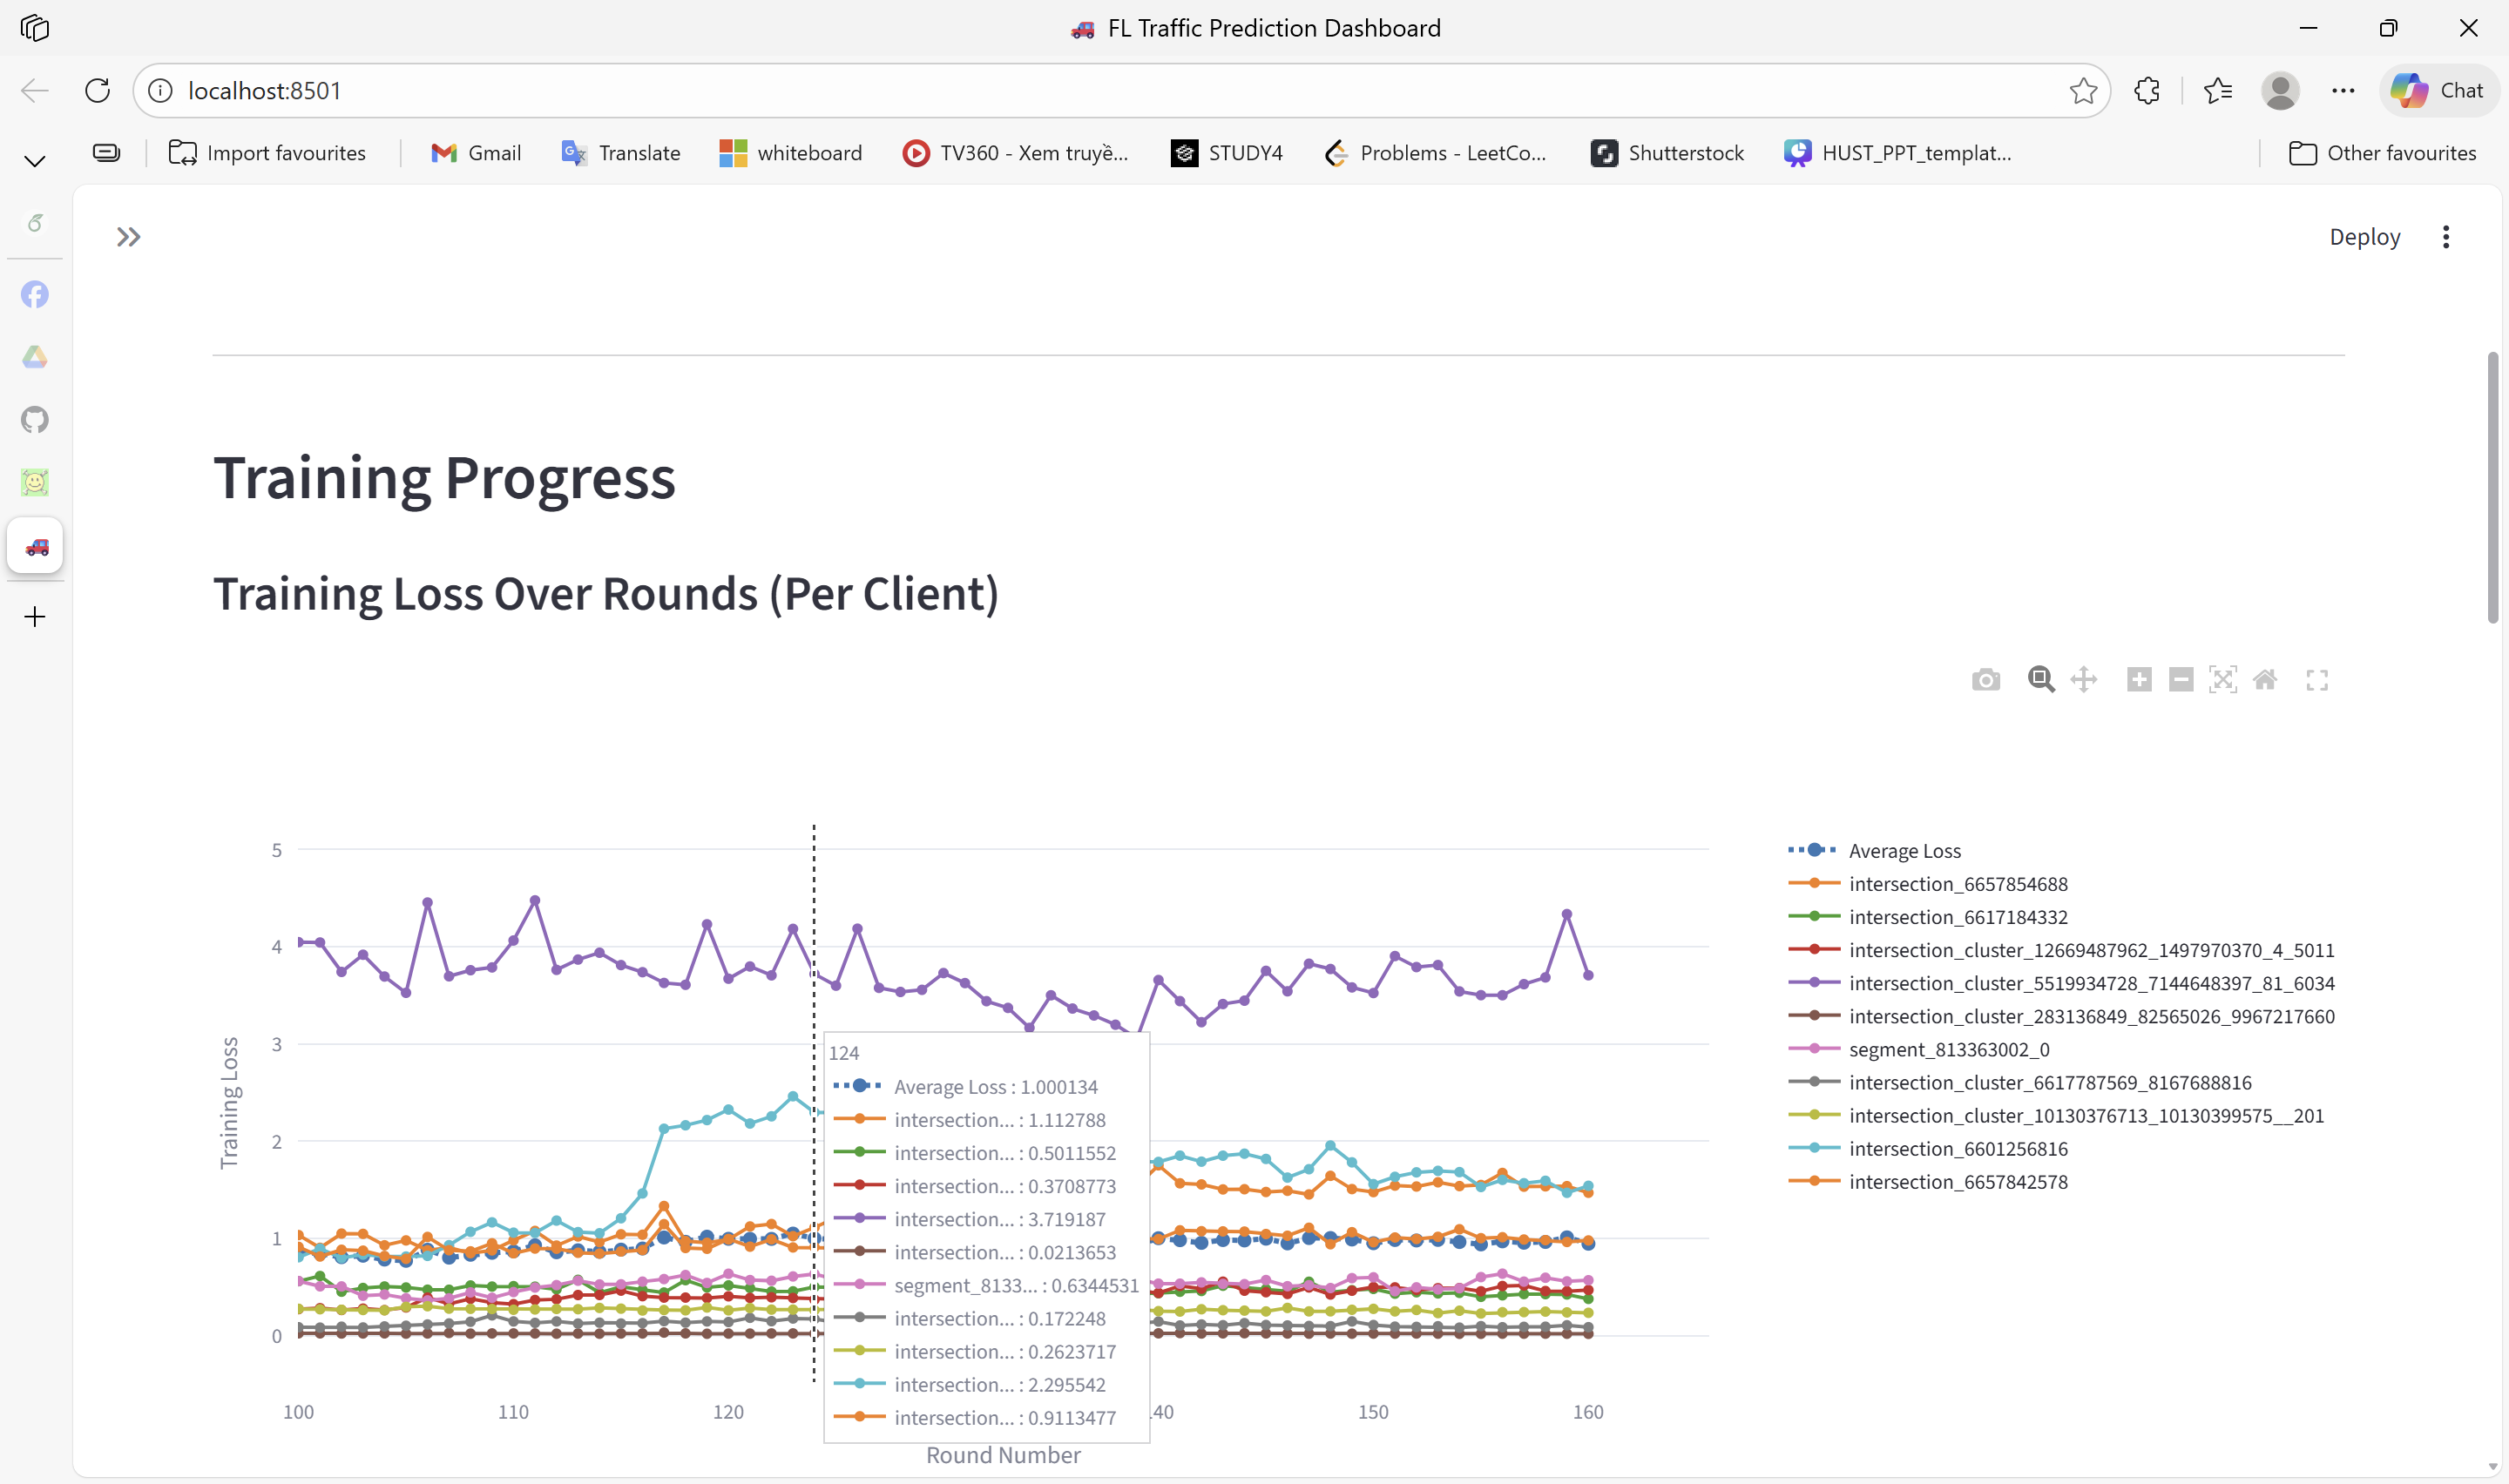
\includegraphics[width=1.0\textwidth]{Figure/dashboard-training-loss.png}
    \caption{Training Loss Over Rounds (Per Client). }
    \label{fig:dashboard_training_loss}
\end{figure}

The dashboard also provides filtering options, client selection for focused monitoring,
and data export for further analysis. The training loss decreases steadily across 160
rounds for 10 different edge clients, indicating successful model convergence. While
different clients show varying convergence patterns due to data differences, all remain
stable without divergence, demonstrating effective federated learning.

Key observations from the training loss chart are as follows:

\begin{itemize}
    \item \textbf{Convergence pattern:} There are three distinct phases in the training
    process: a rapid decrease in loss during early rounds, followed by a slower
    improvement phase, and a final plateau where the model converges with minimal
    further improvement.

    \item \textbf{Per-client heterogeneity:} Different clients experience varying
    convergence behavior due to differences in traffic conditions. Some clients reach
    stable loss more quickly, while others fluctuate due to non-recurring congestion
    events. Despite this, all clients inevitably decrease to similar loss levels.

    \item \textbf{No divergence:} No client shows unstable or diverging behavior,
    indicating that the federated learning method is robust and all clients remain
    close to the average performance.
\end{itemize}

\begin{figure}[H]
    \centering
    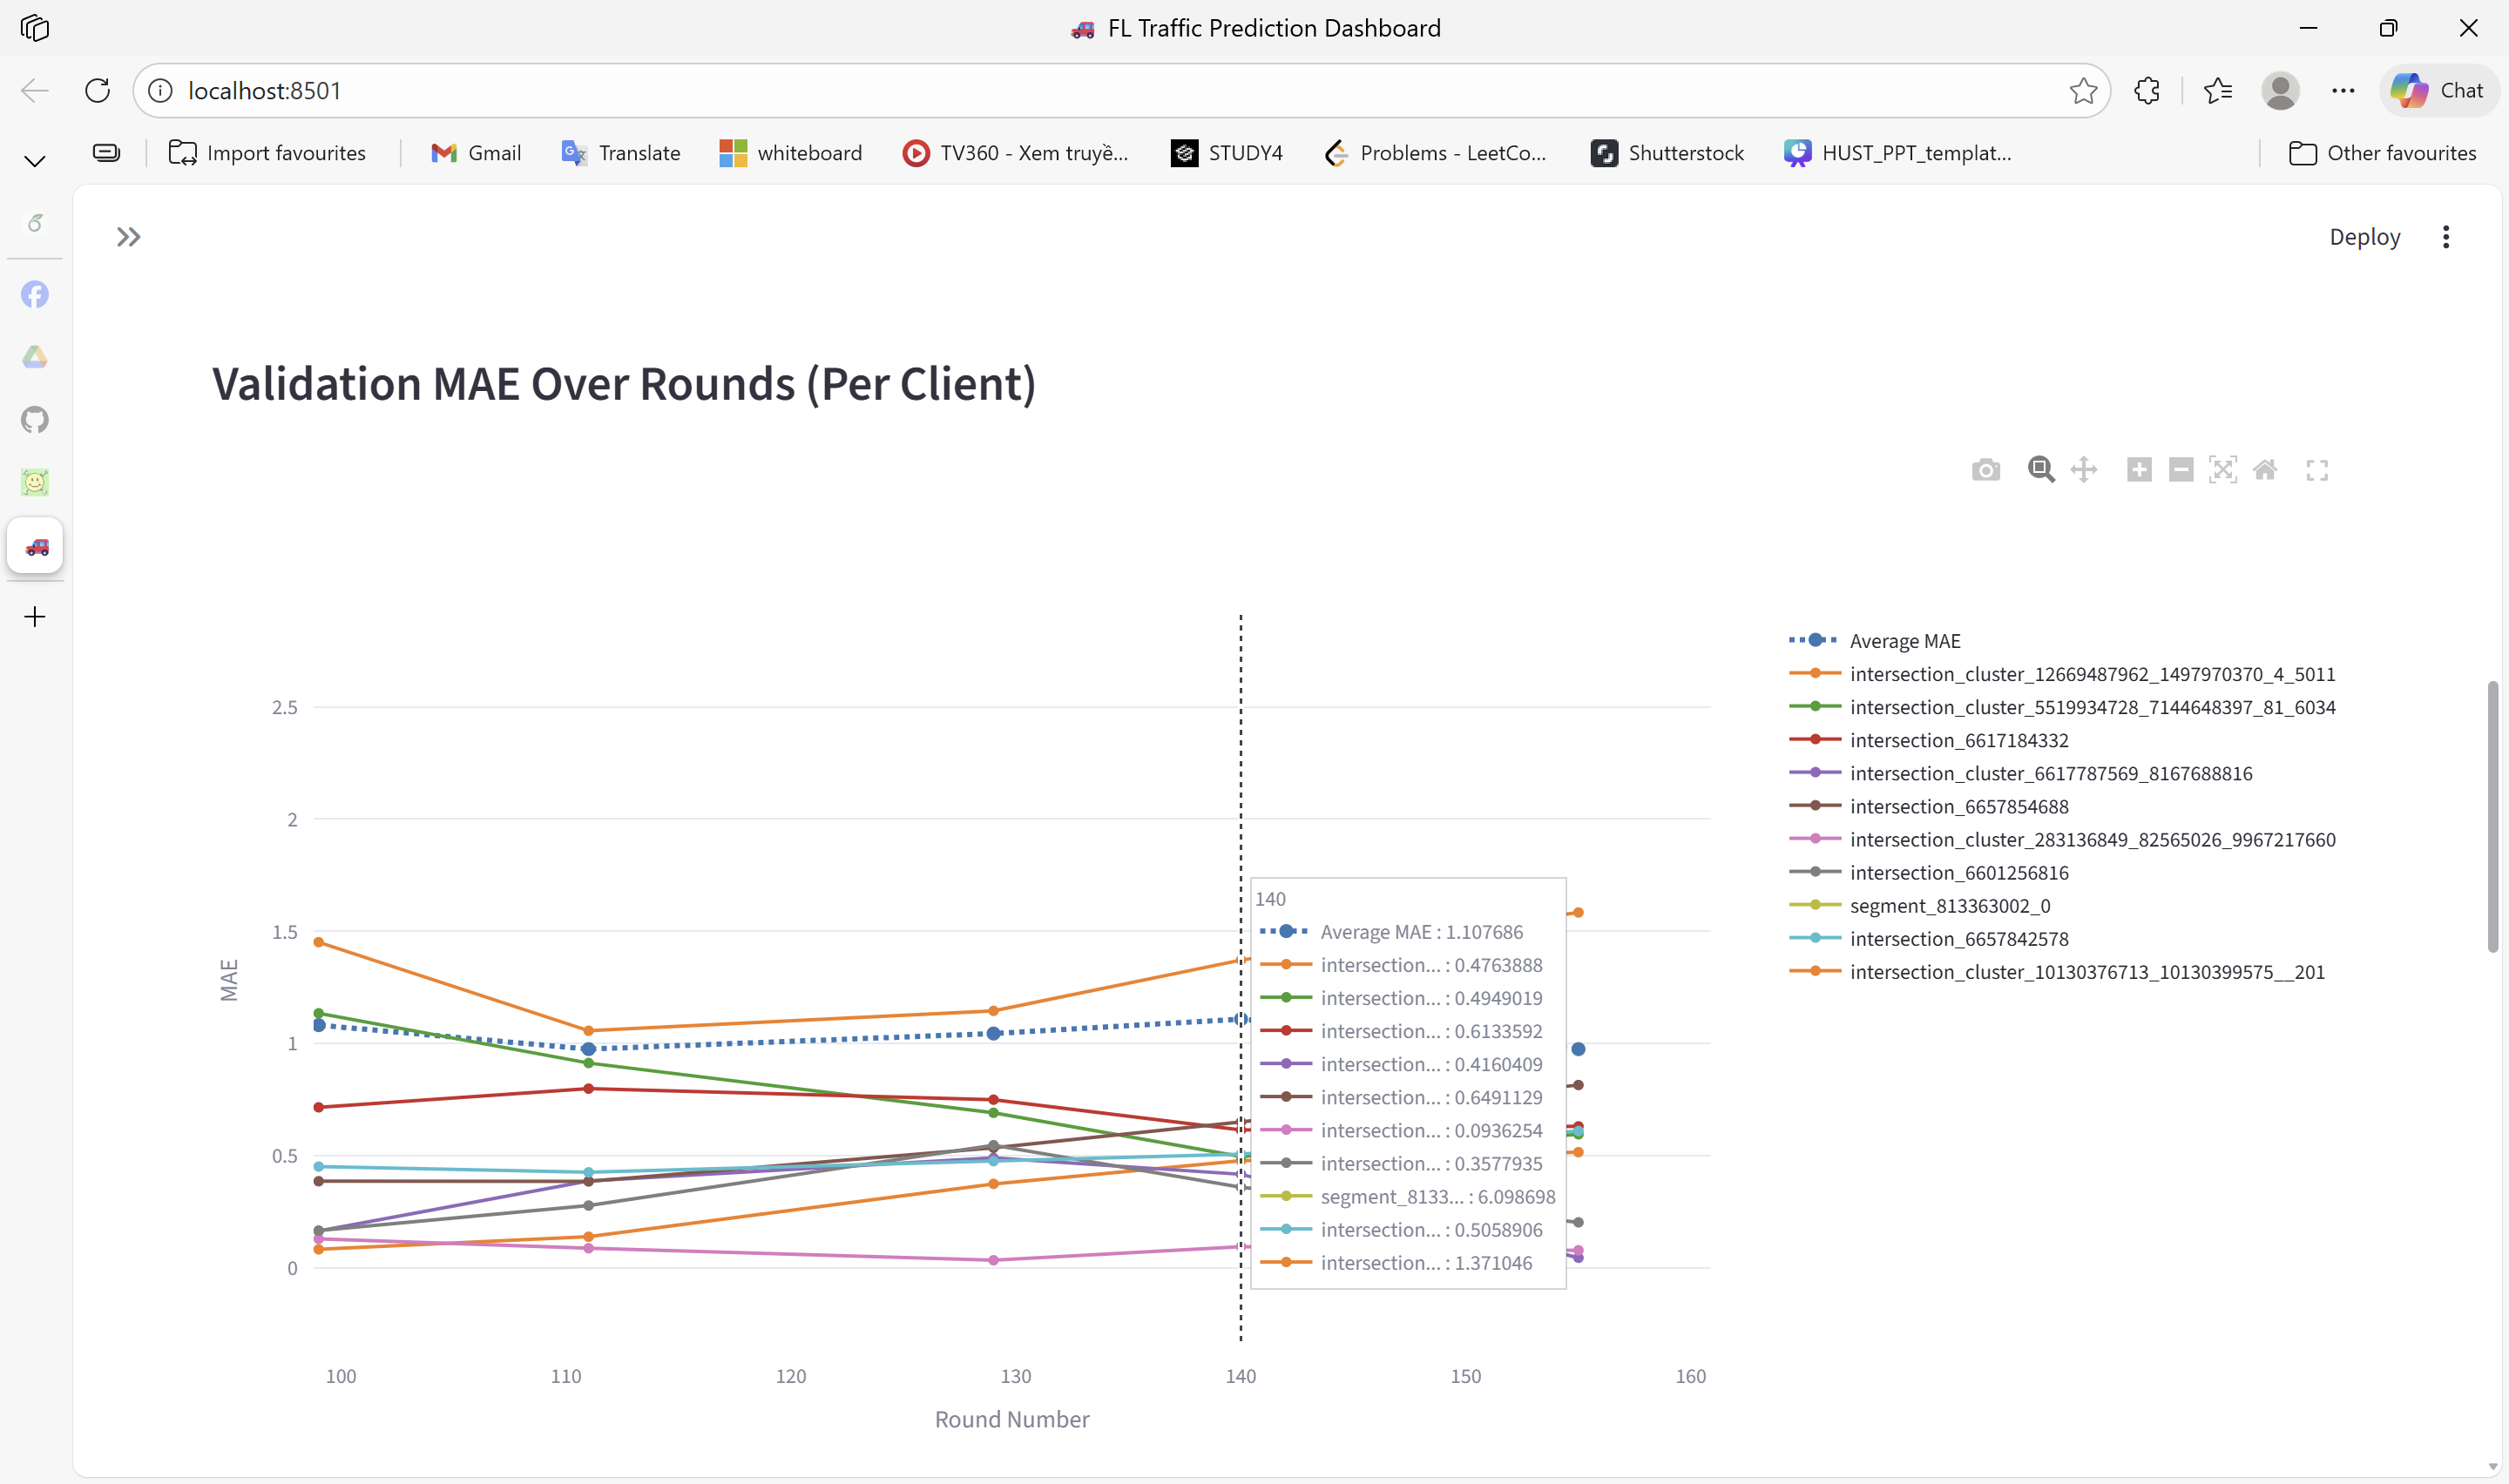
\includegraphics[width=1.0\textwidth]{Figure/dashboard-validation-mae.png}
    \caption{Validation MAE Over Rounds (Per Client). }
    \label{fig:dashboard_validation_mae}
\end{figure}

The validation MAE decreases over training rounds, showing continuous improvement
of the model. Different clients achieve different levels of accuracy depending on traffic
complexity, with some performing better in predictable environments and others showing
higher error in more complex regions. The differences in MAE across all clients
demonstrates that federated learning preserves regional specialization while enabling
global knowledge sharing.

Analysis of validation MAE:

\begin{itemize}
    \item \textbf{Accuracy range:} Validation accuracy varies across clients depending
    on traffic complexity. Clients in predictable environments achieve low error, while
    those in more complex or congested areas exhibit higher error.

    \item \textbf{Monotonic improvements:} All clients show a general decrease in
    validation error over time, indicating consistent improvement. This confirms that
    global model updates benefit all clients, local training is effective, and no client
    experiences performance degradation.

    \item \textbf{Fairness:} The variation in error across clients reflects differences
    in traffic conditions rather than unfairness. Even clients in more difficult
    environments benefit from federated learning, achieving better performance than
    they would with individual local training.
\end{itemize}

\begin{figure}[H]
    \centering
    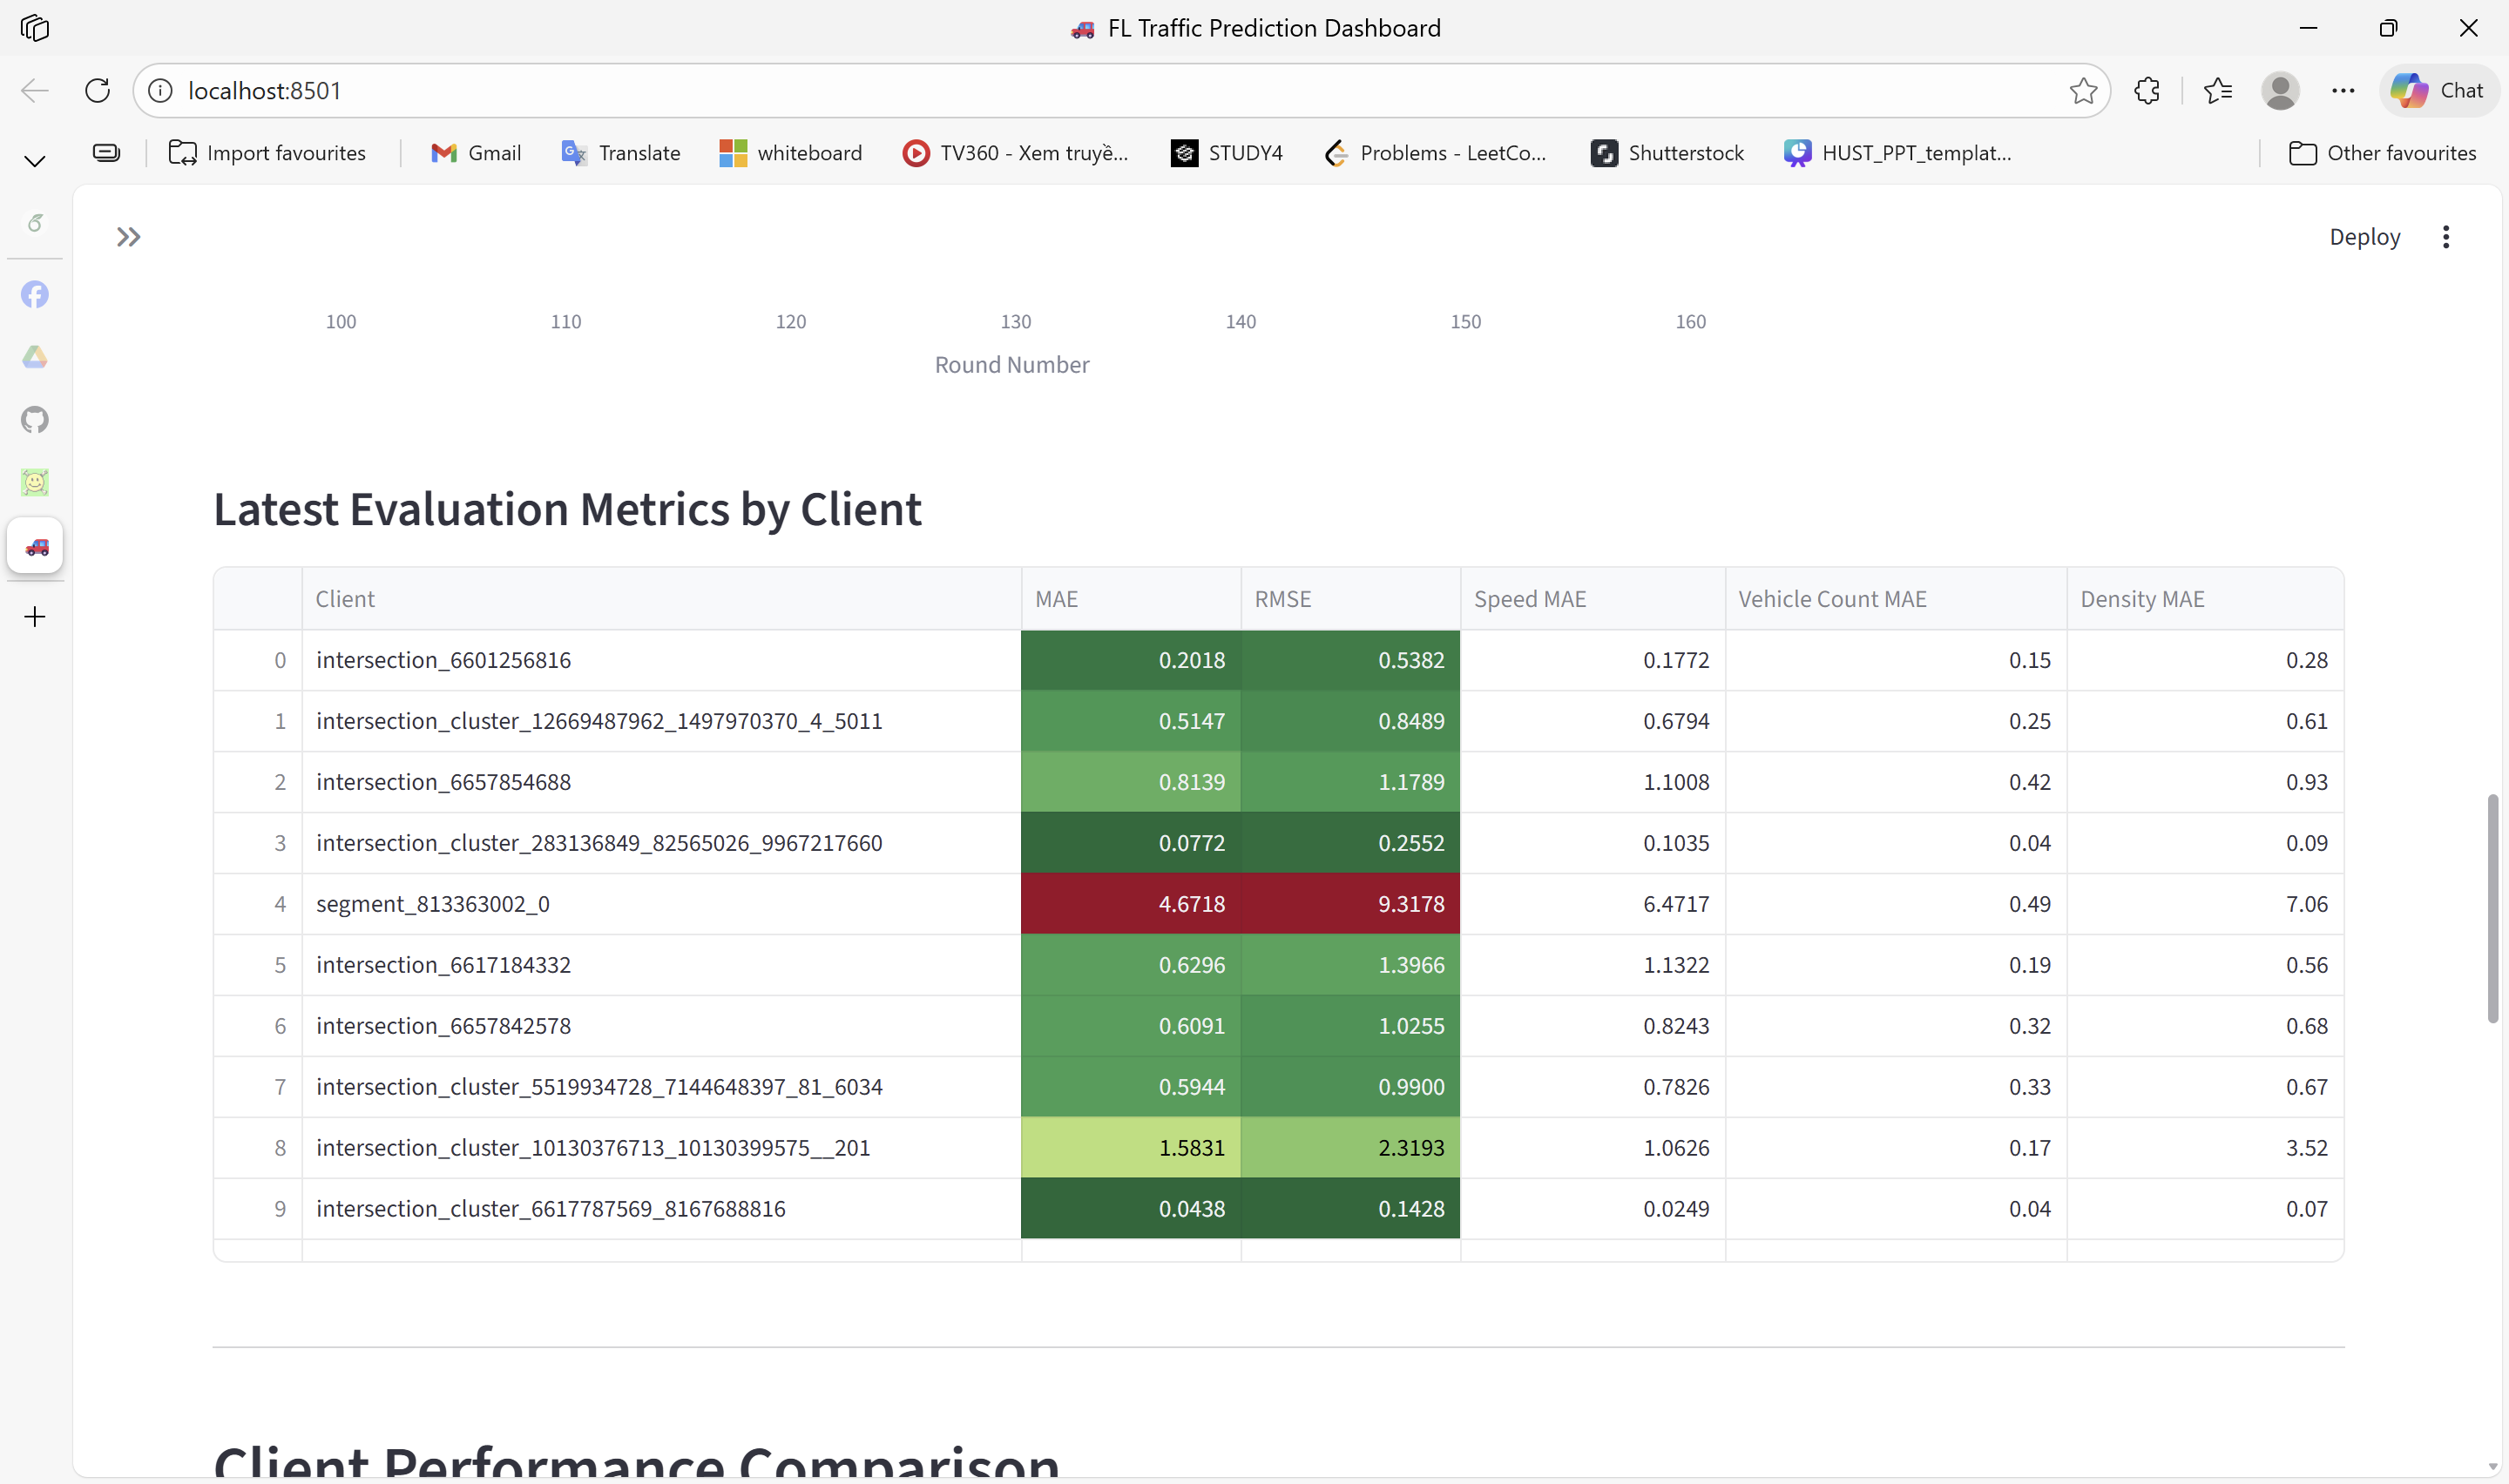
\includegraphics[width=1.0\textwidth]{Figure/dashboard-client-table.png}
    \caption{Latest Evaluation Metrics by Client.}
    \label{fig:dashboard_client_table}
\end{figure}

The per-client metrics table shows that most clients achieve strong performance, while
a few clients in more complex regions have higher error. Overall, the system effectively
handles diverse traffic conditions, with detailed metrics confirming its ability to model
different traffic dynamics across clients. Interpretation of the per-client metrics is as
follows:

\begin{itemize}
    \item \textbf{MAE (Mean Absolute Error):} The main accuracy metric, where lower
    values indicate better performance. Clients 0, 3, and 9 achieved excellent results;
    clients 1--2 and 5--8 showed good or acceptable performance; client 4 is the only
    one with a problematic MAE level.

    \item \textbf{RMSE (Root Mean Squared Error):} An error metric that emphasizes
    larger errors, helping identify outliers. When MAE is close to
    $\text{RMSE}/\sqrt{3}$, errors are consistent; a much higher RMSE indicates
    occasional large prediction errors.

    \item \textbf{Speed / Vehicle Count / Density MAE:} Additional MAE metrics that
    provide detailed information about model performance across individual traffic
    features.
\end{itemize}

% =========================
% SECTION 4.2
% =========================
\section{Evaluation Metrics}

The model performance is evaluated using three standard regression metrics: MAE,
RMSE, and MAPE, defined as follows.

\textbf{Mean Absolute Error (MAE)} measures the average magnitude of prediction
errors without considering direction:
\begin{equation}
    \text{MAE} = \frac{1}{n} \sum_{i=1}^{n} \left| \hat{y}_i - y_i \right|
    \label{eq:mae}
\end{equation}

\textbf{Root Mean Squared Error (RMSE)} penalizes larger errors more heavily by
squaring the residuals before averaging:
\begin{equation}
    \text{RMSE} = \sqrt{\frac{1}{n} \sum_{i=1}^{n} \left( \hat{y}_i - y_i \right)^2}
    \label{eq:rmse}
\end{equation}

\textbf{Mean Absolute Percentage Error (MAPE)} expresses the average error as a
percentage of the true values, enabling scale-independent comparison:
\begin{equation}
    \text{MAPE} = \frac{1}{n} \sum_{i=1}^{n} \left| \frac{\hat{y}_i - y_i}{y_i} \right| \times 100\%
    \label{eq:mape}
\end{equation}

\noindent where $y_i$ denotes the ground-truth value, $\hat{y}_i$ denotes the
predicted value, and $n$ is the total number of samples.

% =========================
% SECTION 4.3 (teammate's section — do not edit)
% =========================
\section{Experimental Results on Benchmark Dataset}
\subsection{Convergence Analysis}
\subsection{Multi-Horizon Prediction Performance}
\subsection{Client-Level Performance Analysis}
\subsection{Comparison with Centralized Baseline}

% =========================
% CHAPTER 5
% =========================
\chapter{CONCLUSION AND FUTURE WORK}

\section{Summary}

\section{Future Works}
\subsection{Multimodal Data Fusion: Cameras and Weather}
\subsection{Multimodal Fusion Strategies}
\subsection{Data Engineering and Collection}

% =========================
% REFERENCES
% =========================
\bibliographystyle{plain}
\bibliography{sn-bibliography}

\end{document}